\chapter{Attachments}

\section{Documentation}\label{sec:documentation}

% https://osmfoundation.org/wiki/Licence/Attribution_Guidelines#Static_images

The project documentation comprises the following \emph{three} parts.

\begin{description}
\item[User's documentation] gives an overview of how to use the application and~ac\-com\-plish basic tasks, such as searching for and managing entities.\\[0.2em] \emph{Please note that this is a simplified version of Attachment~\ref{sec:use-cases-attached} with~screen\-shots. Examples of the user interface are depicted in Figures~\ref{fig:uc04-search-routes-config} and~\ref{fig:uc04-search-routes-result}.}
\item[Programmer's guide] brings clarity into the application architecture and code organization.\\[0.2em]
\emph{Please note that this is a condensed version of Section~\ref{sec:architecture} and Chapter~\ref{chap:implementation}.}
\item[Administrator's guide] provides instructions for preparing a dataset, running the application in development or production mode on a personal computer, and troubleshooting potential issues.
\end{description}

The version of the documentation at the time of submitting the thesis is avail\-able in the \texttt{./docs/} folder of the electronic attachment, and the latest version is hosted at

\begin{center}
\texttt{\href{https://zhukovdm.github.io/smartwalk-docs/}{https://zhukovdm.github.io/smartwalk-docs/}}.
\end{center}

\section{Prerequisites}\label{sec:prerequisites}

\emph{SmartWalk} is essentially cross-platform. However, Unix utilities simplify certain aspects of system maintenance. We assume that the application will run on \emph{Unix-like} environments, such as Linux or Windows Subsystem for Linux\footnote{\href{https://learn.microsoft.com/en-us/windows/wsl/about}{https://learn.microsoft.com/en-us/windows/wsl/about}}.

Please ensure that the following programs are installed on the target system. If mentioned, \underline{preserve} versions of packages due to library dependencies.

\begin{itemize}
\item Docker
\item .NET SDK, v6.0
\item Git
\item GNU Bash, Make, Tar, and Wget
\item Node.js, v18.x (install via nvm\footnote{\href{https://github.com/nvm-sh/nvm\#install--update-script}{https://github.com/nvm-sh/nvm\#install--update-script}})
\end{itemize}

Clone the repository with \emph{submodules} and navigate to its root folder:

\begin{minted}[fontsize=\footnotesize]{text}
$ git clone --recurse-submodules https://github.com/zhukovdm/smartwalk.git
$ cd ./smartwalk/
\end{minted}

\clearpage

\begin{figure}
  \centering
  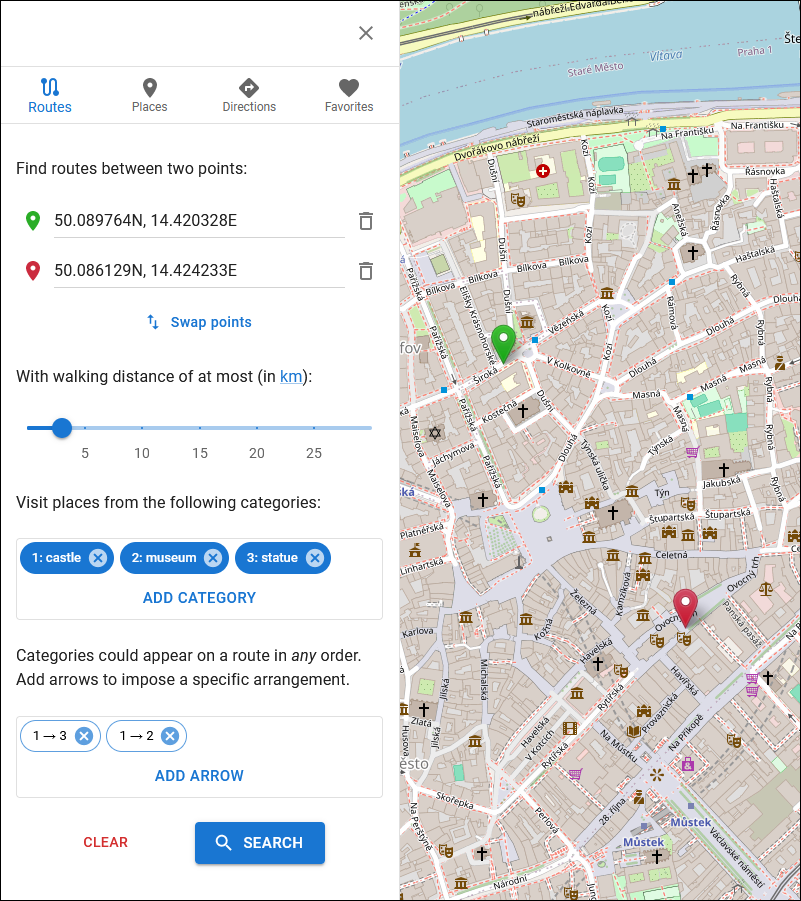
\includegraphics[width=1.00\linewidth]{img/attach/uc04-search-routes-config.png}
  \caption{The panel for searching routes with configured input parameters.}
  \label{fig:uc04-search-routes-config}
\end{figure}

\clearpage

\begin{figure}
  \centering
  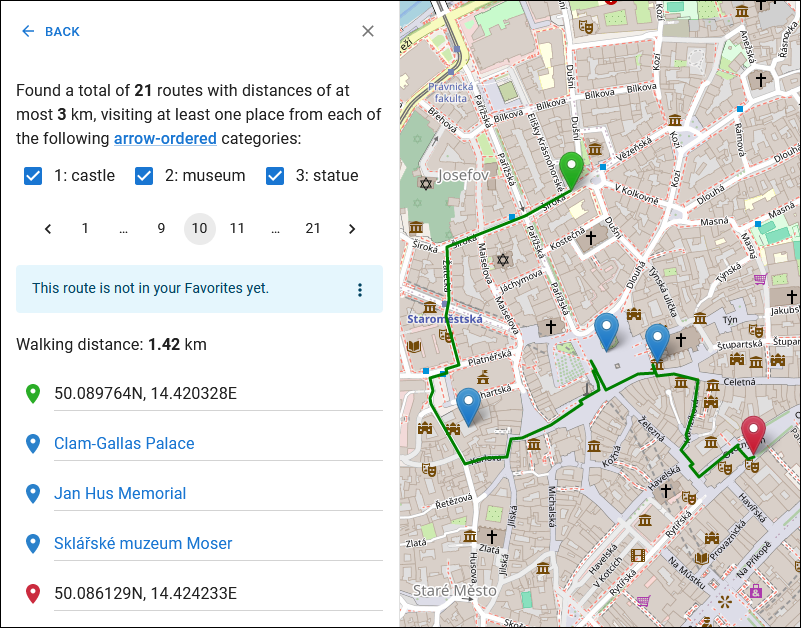
\includegraphics[width=1.00\linewidth]{img/attach/uc04-search-routes-result.png}
  \caption{The results of a route search.}
  \label{fig:uc04-search-routes-result}
\end{figure}

\clearpage

\section{Use cases}\label{sec:use-cases-attached}

\subsection{UC01: Select point}\label{sssec:uc-select-point}

\uctitle{Initial state}

\begin{ucitemize}
\item A user has opened a panel for searching routes, places, or directions.
\end{ucitemize}

\uctitle{Normal flow}

\begin{ucenumerate}
\item The user clicks the ``Select point'' button to fill the corresponding slot.
\item The system shows a dialog with two options:
\begin{ucenumerate}
\item select a location on the map,
\item select a place from the list of stored places.
\end{ucenumerate}
\item The user performs one of the following workflows.
\begin{itemize}
\item They vote for option (a).
\begin{ucenumerate}[label=\roman*.]
\item The user clicks the button ``Select location''.
\item The system hides the panel and dialog, presenting only the map.
\item The user selects a location by clicking on the map.
\end{ucenumerate}
\item They vote for option (b).
\begin{ucenumerate}[label=\roman*.]
\item The user selects a place from the list of stored places and confirms their choice.
\end{ucenumerate}
\end{itemize}
\end{ucenumerate}

\uctitle{Final state}

\begin{ucitemize}
\item The panel appears with the selected entity set as required.
\end{ucitemize}

\subsection{UC02: Add category}\label{sssec:uc-add-category}

\uctitle{Initial state}

\begin{ucitemize}
\item A user has navigated to a panel for searching routes or places.
\end{ucitemize}

\uctitle{Normal flow}

\begin{ucenumerate}
\item The user clicks on the ``Add category'' button.
\item The application opens the dialog and proposes to type in a keyword.
\item The user starts typing. For every prefix, the system suggests options.
\item The user clicks on one of the options confirming their choice.
\item The system shows keyword-specific attribute filters below the input field.
\item The user activates attribute filters relevant to their search and sets bounds.
\item The user clicks on the ``Confirm'' button once the desired configuration has been achieved.
\end{ucenumerate}

\uctitle{Final state}

\begin{ucitemize}
\item The newly created category is appended to the list.
\end{ucitemize}

\uctitle{Alternatives}

\begin{ucitemize}
\item The system raises an error upon a failed attempt to suggest options.
\end{ucitemize}

\uctitle{Extensions}

\begin{ucitemize}
\item The configuration of the attribute filters of a category can be altered at any time by clicking on the category element and applying changes.
\end{ucitemize}

\subsection{UC03: Add arrow}\label{sssec:uc-add-arrow}

\uctitle{Initial state}

\begin{ucitemize}
\item A user has navigated to the panel for searching routes.
\end{ucitemize}

\uctitle{Normal flow}

\begin{ucenumerate}
\item The user clicks on the ``Add arrow'' button.
\item The application opens the dialog, shows the current precedence graph, and proposes to add a new arrow.
\item The user selects the left and right counterparts of the arrow and clicks on the ``Confirm'' button.
\end{ucenumerate}

\uctitle{Final state}

\begin{ucitemize}
\item The newly created arrow is appended to the list.
\end{ucitemize}

\uctitle{Alternatives}

\begin{ucitemize}
\item The system raises an error if the user attempts to create a cyclic dependency or repeats an existing arrow.
\end{ucitemize}

\subsection{UC04: Search routes}\label{sssec:uc-search-routes}

\uctitle{Initial state}

\begin{ucitemize}
\item A user has navigated to the panel for searching routes.
\end{ucitemize}

\uctitle{Normal flow}

\begin{ucenumerate}
\item The user performs the following steps:
\begin{ucitemize}
\item Select a starting point and a destination following \emph{\nameref{sssec:uc-select-point}}.
\item Set a maximum walking distance using the corresponding slider.
\item Configure a non-empty list of categories applying \emph{\nameref{sssec:uc-add-category}} repeatedly.
\item Configure an optional list of arrows applying \emph{\nameref{sssec:uc-add-arrow}} repeatedly.
\end{ucitemize}
\item The user clicks the ``Search'' button, finalizing their request.
\item The system navigates the user to the panel with a paginated list of routes.
\end{ucenumerate}

\uctitle{Alternatives}

\begin{ucitemize}
\item The system rejects the query if the crow-fly distance between the starting point and destination exceeds the maximum limit.
\item If the system fails to find routes, it proposes to alter search parameters.
\item If the system fails to complete the query, it informs the user via an error.
\end{ucitemize}

\subsection{UC05: Show detailed view of a place}\label{sssec:uc-detailed-view}

\uctitle{Initial state}

\begin{ucitemize}
\item The user has navigated to the detailed view of a place using a link or entered the link directly into the browser.
\end{ucitemize}

\newpage

\uctitle{Normal flow}

\begin{ucenumerate}
\item The system shows a progress spinner and renders the view once the object is ready to be presented.
\end{ucenumerate}

\uctitle{Alternatives}

\begin{ucitemize}
\item An object with the given identifier does not exist, or an error has occurred while retrieving the object. Then, the system informs the user via an alert.
\end{ucitemize}

\subsection{UC06: Save place}\label{sssec:uc-save-place}

\uctitle{Initial state}

\begin{ucitemize}
\item The user has obtained a detailed view of a place that has not been saved.
\end{ucitemize}

\uctitle{Normal flow}

\begin{ucenumerate}
\item The user clicks the ``Menu'' button and then the ``Save'' menu item.
\item The system shows a dialog, proposes to enter metadata of the place and informs that a personal copy is about to be created.
\item The user enters a name and confirms their choice by clicking the ``Confirm'' button.
\end{ucenumerate}

\uctitle{Final state}

\begin{ucitemize}
\item The system updates the private storage, hides the dialog, and marks the place as saved.
\end{ucitemize}

\uctitle{Alternatives}

\begin{ucitemize}
\item The system fails to update the private storage and shows an alert.
\end{ucitemize}

\subsection{UC07: Search directions}\label{sssec:uc-search-direcs}

This use case has many similarities with \emph{\nameref{sssec:uc-search-routes}}. Instead of~pro\-viding its full description, let us cover various options on how to extend a sequence of points depicted in Figure~\ref{fig:uc-search-direcs}. Most of them are implemented to enhance the user experience.

The sequence can be extended by selecting a point directly on the map or~from the private storage using standard \emph{\nameref{sssec:uc-select-point}}. This use case implies that the user interface shows the panel for searching directions.

Nevertheless, the user might want to browse through stored entities to recall the content. The system enables them to append places and move points of paths directly from the storage.

To avoid the overhead of storing and navigating, the user could also modify a route that has appeared in the result of a search query or append a place from its detailed view.

\subsection{UC08: Modify route}\label{sssec:uc-modify-route}

\uctitle{Initial state}

\begin{ucitemize}
\item A user has navigated to the panel with stored entities and sees the route to be modified.
\end{ucitemize}

\uctitle{Normal flow}

\begin{ucenumerate}
\item The user clicks the ``Menu'' button and then the ``Modify'' menu item.
\item The system shows a dialog with the message informing that points of this route will replace those configured in the panel for searching directions.
\item The user clicks the ``Confirm'' button.
\end{ucenumerate}

\uctitle{Final state}

\begin{ucitemize}
\item The system redirects the user to the panel for searching directions. Points of the selected path have replaced old ones.
\end{ucitemize}

\subsection{UC09: View entity}\label{sssec:uc-view-entity}

\uctitle{Initial state}

\begin{ucitemize}
\item A user has navigated to the panel with stored entities and sees the entity to be viewed.
\end{ucitemize}

\uctitle{Normal flow}

\begin{ucenumerate}
\item The user clicks the ``Menu'' button and then the ``View'' menu item.
\end{ucenumerate}

\uctitle{Final state}

\begin{ucitemize}
\item The system immediately redirects the user to the viewer panel.
\end{ucitemize}

\subsection{UC10: Edit entity}\label{sssec:uc-edit-entity}

\uctitle{Initial state}

\begin{ucitemize}
\item A user has navigated to the panel with stored entities and sees the entity to be edited.
\end{ucitemize}

\uctitle{Normal flow}

\begin{ucenumerate}
\item The user clicks the ``Menu'' button and then the ``Edit'' menu item.
\item The system shows a dialog with editable fields containing current metadata.
\item The user sets new values for selected items and clicks the ``Save'' button.
\end{ucenumerate}

\uctitle{Final state}

\begin{ucitemize}
\item The system hides the dialog, indicating that the object has been updated.
\end{ucitemize}

\uctitle{Alternatives}

\begin{ucitemize}
\item The system fails to update the object and shows an alert.
\end{ucitemize}

\subsection{UC11: Activate Solid pod}\label{sssec:uc-activate-solid}

\uctitle{Initial state}

\begin{ucitemize}
\item A user has loaded the initial web page.\\[0.2em]
\emph{A \acs{solid} pod can be activated at any time unless another one is active.}
\end{ucitemize}

\uctitle{Normal flow}

\begin{ucenumerate}
\item The user clicks the ``Log In'' button outside the panel drawer and then the ``Solid'' menu item.
\item The system shows a dialog with an input field and asks to enter the URL of a \acs{solid} pod provider.
\item The user enters the URL or selects from the list and then clicks the ``Log In'' button.
\item The system redirects to the web page of the selected pod provider so that the user can enter their credentials and allow the application to access pods.
\item The user is redirected to the initial web page, and the ``Solid'' panel opens up shortly after.
\item The user selects a pod from the list of pods associated with their account and clicks the ``Activate Pod'' button.\\[0.2em]
\emph{Before this step, the application still uses entities from the device storage.}
\item The system redirects to the panel with stored entities, and loads the content from the \acs{solid} pod.
\end{ucenumerate}

\uctitle{Final state}

\begin{ucitemize}
\item The user ends up in the panel with entities stored in the activated pod.
\end{ucitemize}

\uctitle{Alternatives}

\begin{ucitemize}
\item The system fails to activate pod and shows an error. No redirection to the panel with stored entities occurs.
\item The system fails to load the content of the activated pod. It shows an error, and the loading spinner remains forever. The user should refresh the web page so that the application can load entities from the device storage.
\end{ucitemize}

\subsection{UC12: Deactivate Solid pod}\label{sssec:uc-deactivate-solid}

\uctitle{Initial state}

\begin{ucitemize}
\item The user has activated a pod following \emph{\nameref{sssec:uc-activate-solid}}.
\end{ucitemize}

\uctitle{Normal flow}

\begin{ucenumerate}
\item The user clicks the ``Solid'' button outside the panel drawer so that the system redirects them to the ``Solid'' panel.
\item The user clicks the ``Log Out'' button.
\item The system redirects to the panel with stored entities, and loads the content from the device storage.
\end{ucenumerate}

\uctitle{Final state}

\begin{ucitemize}
\item The user ends up in the panel with entities stored in the device storage.
\end{ucitemize}

\section{Results of usability testing}\label{sec:results-usability-testing}

% CZ: https://forms.gle/FsdJwpC13AdbXzBw9
% EN: https://forms.gle/XPS6Z2yfSidQ9dTQ9
% RU: https://forms.gle/YFgDWcipBxxbZJbAA

The respondents were asked to express their opinions on the following statements, which first appeared in \cite{brooke96}.

\begin{enumerate}[label=\textbf{S\arabic*}]
\item\label{itm:sus-01} I think that I would like to use this system frequently.
\item\label{itm:sus-02} I found the system unnecessarily complex.
\item\label{itm:sus-03} I thought the system was easy to use.
\item\label{itm:sus-04} I think that I would need the support of a technical person to be able to use this system.
\item\label{itm:sus-05} I found the various functions in this system were well integrated.
\item\label{itm:sus-06} I thought there was too much inconsistency in this system.
\item\label{itm:sus-07} I would imagine that most people would learn to use this system very quickly.
\item\label{itm:sus-08} I found the system very cumbersome to use.
\item\label{itm:sus-09} I felt very confident using the system.
\item\label{itm:sus-10} I needed to learn a lot of things before I could get going with this system.
\end{enumerate}

Responses were evaluated on a scale of 1 (strongly disagree) to 5 (strongly agree). Individual scores were calculated using the formula

\begin{equation*}
2.5 \cdot \left( \sum_{i \in \{ 1, 3, 5, 7, 9 \}} \left( S_{i} - 1 \right) + \sum_{j \in \{ 2, 4, 6, 8, 10 \}} \left( 5 - S_{j} \right) \right)
\end{equation*}

and then averaged.

\bgroup
\def\arraystretch{1.2}
\begin{table}[!h]
\centering\footnotesize
\begin{tabular}{ c c c c c c c c c c c c }
\toprule
\textbf{Resp.}
  & \ref{itm:sus-01}
    & \ref{itm:sus-02}
      & \ref{itm:sus-03}
        & \ref{itm:sus-04}
          & \ref{itm:sus-05}
            & \ref{itm:sus-06}
              & \ref{itm:sus-07}
                & \ref{itm:sus-08}
                  & \ref{itm:sus-09}
                    & \ref{itm:sus-10}
                      & \textbf{Score} \\
\midrule
1 & 5 & 1 & 5 & 1 & 5 & 1 & 5 & 2 & 4 & 1 & 95.00           \\
2 & 4 & 2 & 5 & 1 & 3 & 2 & 4 & 1 & 5 & 2 & 82.50           \\
3 & 3 & 2 & 3 & 4 & 5 & 2 & 5 & 2 & 3 & 1 & 70.00           \\
4 & 5 & 1 & 4 & 2 & 5 & 1 & 5 & 1 & 4 & 1 & 92.50           \\
\midrule
  &   &   &   &   &   &   &   &   &   &   & \textbf{85.00}  \\
\toprule
\end{tabular}
\caption{Results of usability testing.}
\label{tab:results-usability-testing}
\end{table}
\egroup

\section{Electronic attachment}\label{sec:electronic-attachment}

The electronic attachment to the thesis follows the structure below.

\begin{description}[font=\tt]
\item[code/] contains source code of the application (tag \href{https://github.com/zhukovdm/smartwalk/releases/tag/v1.0.0}{\texttt{v1.0.0}} on GitHub) and doc\-u\-men\-ta\-tion (tag \href{https://github.com/zhukovdm/smartwalk-docs/releases/tag/v1.0.0}{\texttt{v1.0.0}} on GitHub).
\item[docs/] contains generated documentation for the tag \href{https://github.com/zhukovdm/smartwalk-docs/releases/tag/v1.0.0}{\texttt{v1.0.0}} on GitHub. The file \texttt{./index.html} represents the main page.
\item[perf/] accommodates the dataset, two files \texttt{place.txt} and \texttt{keyword.txt}, for~per\-for\-mance tests we mentioned in Section~\ref{sec:perf-testing}.
\end{description}

% \dirtree{%
%   .1 {1/}.
%   .2 {2/}.
%   .3 {3/}.
%   .4 {4/}.
% }
